\section{Problema 1}
Tomando el número de onda tridimensional $\vec{k} = k_x \vx + k_y \vy + k_z \vz = \frac{\pi}{L}\qty(n_x \vx + n_y \vy + n_z \vz)$, cuya norma $k_n = \frac{\pi}{L} \sqrt{n_x ^2 n_y ^2 n_z ^2} = \frac{\pi}{L} n$. Tomando las coordenadas en terminos de coordenadas esféricas, calculámos el número de puntos entre $n$ y $n+\dd{n} = \overset{\sim}{g} (n) \dd{n}$. Integrando
	$$
		\overset{\sim}{g} (n) \dd{n} = \qty(\int _0 ^{\flatfrac{\pi}{2}} \int _0 ^{\flatfrac{\pi}{2}} n^2 \sin{\theta} \dd{\phi} \dd{\theta}) \dd{n} = \frac{\pi}{2} n^2 \dd{n}.
	$$
Dado que $E_n = \hbar \omega = \frac{\hbar \pi c}{L} n$, entonces $n = \frac{L \omega}{\pi c} \dd{n} = \frac{L}{\pi c} \dd{\omega}$ sustituyendo en lo anterior
	$$
		g(\omega) \dd{\omega} = 2\qty(\frac{\pi}{2} \frac{L^2 \omega ^2}{\pi ^2 c^2} \frac{L}{\pi c} \dd{\omega}) = \frac{L^3 \omega ^2}{\pi ^2 c^3} \dd{\omega};	
	$$
por lo tanto, 
	$$ \boxed{ g(\omega) = \frac{V \omega ^2}{\pi^2 c^3} } $$

\section{Problema 2}
Utilizando la distribución de Bose$-$Einstein
	$$ \frac{n_i}{g_i} = \sum _{i = 1} ^k \frac{1}{e^{\beta (E_i - \mu)} - 1} \qquad \qquad \Rightarrow \qquad \qquad E_T = \sum _{i = 1} ^k \frac{g_i E_i}{e^{\beta (E_i - \mu)} - 1}, $$
entonces, integrando
	$$
		E_T = \int _0 ^\infty \frac{V\hbar \omega ^3 \dd{\omega}}{\pi ^2 c^3 \qty(e^{\beta \hbar \omega} - 1)}.
	$$
Utilizando la serie geométrica reescribimos la integral de la siguiente forma
	$$
		\int _0 ^\infty \frac{\omega ^3 \dd{\omega}}{e^{\beta \hbar \omega} - 1} = \sum _{k = 0} ^\infty \int _0 ^\infty \omega ^3 e^{-\beta \hbar \omega (k + 1)} = \sum _{k = 0} ^\infty \frac{1}{\beta ^4 \hbar ^4 (k+1)^4} \int _0 ^\infty y^{4 - 1} e^{-y} \dd{y}.
	$$
Utilizando la función Gamma y la función zeta de Riemann valuadas en $4$.
	$$ = \frac{1}{\beta ^4 \hbar ^4} \frac{\pi ^4}{15}, $$
entonces
	$$ \boxed{E_T = \frac{V\pi ^2}{15\hbar ^3 c^3 \beta ^4} = \qty(\frac{V\pi ^2 k_B ^4}{15\hbar ^3 c^3})T^4} .$$
	
Encontramos la función espectral de densidad de energía volumétrica, de modo que
	$$ e = \frac{\hbar}{\pi ^2 c^3} \int _0 ^\infty \underbrace{\frac{\omega ^3}{e^{\beta \hbar \omega} - 1}}_{\mu (\omega)} \dd{\omega}, $$
entonces
\begin{equation}
	\boxed{ \mu (\omega) = \frac{\hbar \omega ^3}{\pi ^2 c^3 \qty(e^{\beta \hbar \omega} - 1)} }. \label{muomega}
\end{equation}

Ahora, tomando $\omega = 2\pi \nu$, $\lambda \nu = c$ y $h = 2\pi \hbar$, sustituyendo
\begin{equation}
		\boxed{ \mu (\nu) = \frac{8\pi h \nu ^3}{c^3 \qty(e^{\beta h \nu} - 1)} }	\label{munu}
\end{equation}

y
\begin{equation}
		\boxed{ \mu (\lambda) = \frac{8\pi h}{\lambda^3 \qty(e^{\frac{\beta h c}{\lambda}} - 1)} }	\label{mulambda}
\end{equation}

\section{Problema 3}
Tomando todas las constantes igual a $1$, para facilitar la graficación, de modo que los números de los ejes de las gráficas no significan nada, únicamente la "forma" de la gráfica.

\begin{multicols}{2}
\begin{figure}[H]
	\centering
	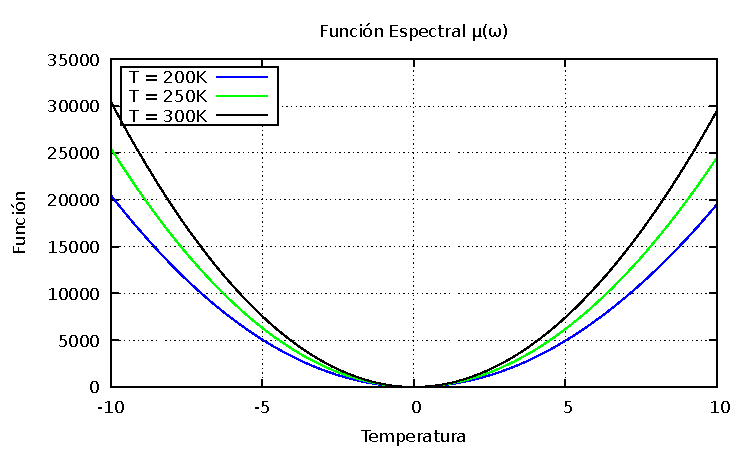
\includegraphics[scale=0.65]{Images/omega.pdf}
	\caption{Gráfica de la ecuación \eqref{muomega}.}
	\label{gmuomega}
\end{figure}

\begin{figure}[H]
	\centering
	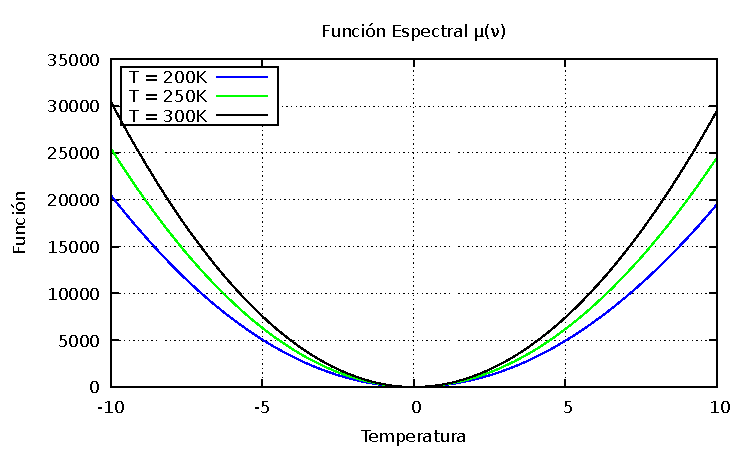
\includegraphics[scale=0.65]{Images/nu.pdf}
	\caption{Gráfica de la ecuación \eqref{munu}.}
	\label{gmunu}
\end{figure}
\end{multicols}

\begin{figure}[H]
	\centering
	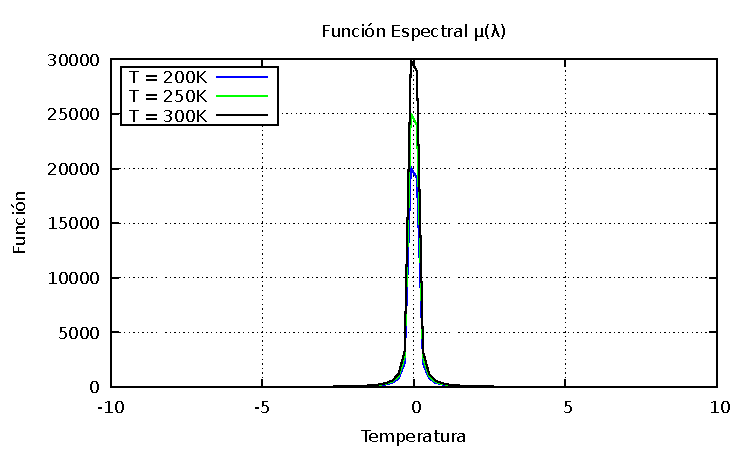
\includegraphics[scale=0.65]{Images/lambda.pdf}
	\caption{Gráfica de la ecuación \eqref{mulambda}.}
	\label{gmulambda}
\end{figure}

\section{Problema 4}
Dado que
	$$ \ln{Z} = \frac{V\pi ^2 k_B ^3 T^3}{45 \hbar ^3 c^3}, $$
entonces, para la energía libre de Helmholtz $A = -\flatfrac{\ln{Z}}{\beta}$, reescribiento un poco lo anterior se tiene
	$$ \boxed{ A = -\frac{4VT^4}{3(60)} \frac{1}{c} \frac{k_B ^4 \pi ^2}{\hbar ^3 c^2} = -\frac{4V\sigma T^4}{3c} }. $$
Ahora, tomando la entroía $S = k_B (\beta E_T + \ln{Z})$, con $\dv{\ln{Z}}{\beta} = -E_T$. Entonces
	$$ \boxed{ S = k_B \qty(\frac{3V\pi^2}{45\hbar ^3 c^3 \beta ^3} + \frac{V\pi^2}{45 \hbar ^3 c^3 \beta ^3}) = \frac{16}{3(60)} \frac{V\pi^2 k_B ^4 T^4}{\hbar ^3 c^3} = \frac{16V\sigma T^4}{3c} }. $$

\section{Problema 5}
Realizando lo mismo que en el problema $2$, solo que para $z = 3$, de modo que 		$$ \int _0 ^\infty \frac{\omega ^2}{e^{\beta \hbar \omega} - 1} \dd{\omega} = \sum _{k = 0} ^\infty \frac{1}{\beta ^3 \hbar ^3 (k + 1)^3} \int _0 ^\infty y^{3 - 1} e^{-y} \dd{y} = \frac{1}{\beta ^3 \hbar ^3} \zeta (3) \Gamma (3) = \frac{2\zeta (3)}{\beta ^3 \hbar ^3} \zeta (3), $$
entonces,
	$$ \boxed{ N = \frac{2\zeta (3) k_B ^3 T^3 V}{\pi ^2 \hbar ^3 c^3} } $$
Tomando la energía promedio $\varepsilon = \flatfrac{E_T}{N}$, entonces, sustituyendo las expresiones y simplificando
	$$ \boxed{ \varepsilon = \frac{\pi ^4 k_B T}{30 \zeta (3)} = 2.70k_B T } $$












%%%%%
